\documentclass[18pt]{beamer}
%% SLIDE FORMAT
\usetheme{Boadilla}
\usepackage[utf8]{inputenc}
\usepackage{algpseudocode}
\usepackage{multicol}

\title[Programmieren Tutorium]{9. Programmieren Tutorium:\texorpdfstring{\\}{} Exceptions}
%\subtitle{Fancy Stuff}
\author{Konstantin Zangerle \texorpdfstring{\\}{} info@konstantinzangerle.de}
\date{18. Jan 2016}

\usepackage{listings}
\usepackage{xcolor}

\setlength\columnseprule{.4pt}

\definecolor{mygreen}{rgb}{0,0.6,0}
\definecolor{mygray}{rgb}{0.5,0.5,0.5}
\definecolor{mymauve}{rgb}{0.58,0,0.82}

\lstset{ %
  backgroundcolor=\color{white},   % choose the background color
  basicstyle=\footnotesize,        % size of fonts used for the code
  breaklines=true,                 % automatic line breaking only at whitespace
  captionpos=b,                    % sets the caption-position to bottom
  commentstyle=\color{mygreen},    % comment style
  escapeinside={\%*}{*)},          % if you want to add LaTeX within your code
  keywordstyle=\color{blue},       % keyword style
  stringstyle=\color{mymauve},     % string literal style
  showstringspaces=false,
  language=Java
}
\beamersetuncovermixins{\opaqueness<1>{0}}{\opaqueness<2->{0}} %Dont show things after pause 
% Bibliography

\begin{document}

% change the following line to "ngerman" for German style date and logos
%\selectlanguage{ngerman}

%title page
\begin{frame}
\titlepage
\end{frame}

%table of contents
\begin{frame}{Gliederung}
\tableofcontents
\end{frame}

\section{Organisatorisches}

\begin{frame}{Weihnachten}
 \begin{itemize}
  \item Erstes Tut im neuen Jahr
  \item Noch Tutorien am 25.01., 1.2, 8.2
 \end{itemize}

\end{frame}





\section{Übungsblatt}
\begin{frame}{Übungsschein}
  \large
  Herzlichen Glückwunsch an alle, die jetzt mehr als 60 Punkte haben.
\end{frame}


\section{Command}

\begin{frame}{Command}
 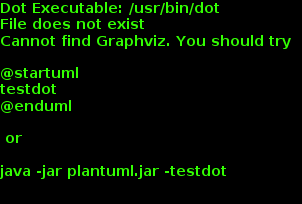
\includegraphics[scale=0.6]{command}
\end{frame}


\begin{frame}{Frohe Weihnachten}
 
 Quelle: http://xkcd.com/835
\end{frame}
\end{document}
